\chapter{Metodologia}
\label{cap:metodologia}

O objetivo geral deste trabalho é realizar uma análise da API do sistema Android a partir de uma análise estática de seu código fonte, e então avaliar a possibilidade de utilizar os resultados como referência para o desenvolvimento de aplicativos desenvolvidos para o Android, partindo da premissa que os aplicativos desenvolvidos utilizando a API do sistema são fortemente dependentes da mesma.

A partir da análise do código fonte, traçar um perfil que caracteriza o próprio sistema a partir de suas métricas de código fonte, assim como traçar esse perfil para os aplicativos do sistema e verificar o grau de aproximação que ambos encontram em seu design. 

Assumindo que o código dos aplicativos do sistema possui uma arquitetura ideal de aplicativos por ser mantido pela Google, bem como pela comunidade de desenvolvedores por ter código aberto, criar um fator de aproximação para aplicar a aplicativos em desenvolvimento para avaliar sua qualidade de acordo com a aproximação ao sistema e à aplicativos nativos, em termos de métricas estáticas de código. Esse fator de aproximação pode ser calculado utilizando métodos estatísticos ou aprendizado de máquina, de forma que possa ser avaliada a aproximação de uma nova amostra aos perfis existentes.

Caso o grau de aproximação de um aplicativo qualquer seja bastante elevado, pode-se inferir uma boa qualidade de código, pelo fato de se aproximar àquelas desenvolvidas pelos próprios arquitetos do sistema.

Utilizar para a análise métricas de código orientado a objetos, bem como outras métricas que refletem decisões arquiteturais e de design. É importante incluir métricas que refletem o volume de código para dar resultados relativos ao tamanho do aplicativo sendo avaliado, uma vez que várias métricas tem seu valor de referência variável de acordo com o tamanho do código. Utilizar valores do sistema, como milhões de linhas de código, como referencia para analisar um aplicativo com apenas algumas centenas de linhas resulta em uma comparação inválida para os valores de algumas métricas, como discutido no Capítulo~\ref{cap:metricas}.

Algumas conclusões talvez já possam ser tiradas de acordo com a aproximação do código do sistema aos aplicativos nativos, caso os mesmos sejam a referencia. Por exemplo, a respeito dos aplicativos nativos, se os resultados mostrarem que nenhum se aproxima a mais de 70\% do sistema, então pode-se inferir que a aproximação ideal ao sistema seja esta, e talvez uma maior que 70 não seja desejada em aplicativos de terceiros. Da mesma forma, uma aproximação muito alta pode indicar a possibilidade de utilizar os valores da mesma como referência, utilizando os aplicativos para gerar mais amostras relativas de tamanho.

\section{Pesquisa}

Baseando-se nas ideias apresentadas, é levantada a seguinte questão de pesquisa:

\begin{itemize}
\item É possível monitorar métricas estáticas de código fonte de aplicativos Android de acordo com a análise e predição da evolução do código do sistema?
%\item É efetivo usar o próprio sistema como arquitetura referência devido ao acoplamento de aplicativos com a própria API de desenvolvimento?
\end{itemize}

Respondendo a essa pergunta podemos confirmar a efetividade de utilizar o próprio sistema como arquitetura referência em análise de aplicativos desenvolvidos para ele.

Para alcançar os objetivos descritos e responder as questões de pesquisa que foram definidas, algumas hipóteses devem ser estudadas e avaliadas:

\begin{itemize}
\item É possível identificar padrões e tendências na evolução da arquitetura do sistema Android e nos aplicativos desenvolvidos para ele.
\item O desenvolvimento de aplicativos Android pode ser guiado pelo resultado de uma análise evolutiva do código do próprio sistema.
\end{itemize}

Como uma hipótese adicional neste trabalho, será avaliado, através da comparação com o sistema, o resultado parcial inicial deste trabalho, que corresponde a um aplicativo Android desenvolvido com o objetivo de criar uma arquitetura modularizada, flexível e manutenível. Foram tomadas diversas decisões teóricas com o objetivo de alcançar a melhor arquitetura para um aplicativo Android desenvolvido para um estudo de caso específico. Surge então uma hipótese adicional, para avaliar se as decisões tomadas com base em experiência de desenvolvedor e padrões de projeto são refletidas e semelhantes as decisões que podem ser tomadas com base em resultados de análise estática de código fonte, como as análises realizadas neste trabalho.

\begin{itemize}
\item As decisões arquiteturais teóricas aplicadas no estudo de caso e-lastic estão relacionadas com decisões arquiteturais baseadas em métricas.
\end{itemize}

O projeto do aplicativo desenvolvido durante o início deste trabalho para esse estudo de caso específico também deve ser submetido a análise de aproximação ao código do sistema e de aplicativos nativos, de forma a validar as decisões tomadas durante o desenvolvimento do mesmo.

\section{Trabalhos relacionados}

\citeonline{androidblackberry}  realiza um estudo de dependência das APIs de desenvolvimento tanto da plataforma Android quanto da plataforma Blackberry, a fim de fazer uma comparação entre os sistemas. A partir disso, é verificado o quanto uma API influencia na quantidade de código desenvolvido, assim como é verificada a dependência de código de terceiros para o desenvolvimento de aplicativos. Em suma, o resultado comparativo demonstrou que aplicativos no sistema Android são significativamente mais dependentes da API do sistema devido a maior completude da API, reduzindo por consequência a quantidade de código de terceiros e código próprio dentro dos projetos. Embora possa tornar mais fácil o desenvolvimento, essa dependência maior em relação ao código do sistema torna o código de aplicativo desenvolvido para Android difícil de ser portado para outras plataformas.

\citeonline{samoa} apresenta o desenvolvimento de uma ferramenta de análise estática de código, que avalia não apenas métricas de código fonte do sistema, como dependência de código de terceiros dentro do projeto de aplicativos Android. O objetivo não é apenas analisar software em plataforma móvel, mas também diferenciar a abordagem quado analisando um software tradicional ou um software para dispositivo móvel, de forma a verificar a manutenibilidade desses sistemas. O estudo de \citeonline{androidblackberry} também apresenta algumas discussões no quesito manutenibilidade em sistemas móveis. Assim como neste último, \citeonline{samoa} demonstra uma alta dependência de aplicativos android em relação ao sistema, apresentando em geral cerca de  2/3 das chamadas de método de aplicativos sendo para bibliotecas externas ao app, em sua maioria para a API Android ou métodos de bibliotecas padrão Java.

\citeonline{evolutionandroid} reforça a idéia de dependência de aplicativos em relação a API Android, e fala sobre as grandes mudanças da API devido a sua rápida evolução nos ultimo anos. Tenta então ajudar desenvolvedores com dicas para melhor se prepararem para mudanças na plataforma, assim como para mudanças em bibliotecas de terceiros, que podem ser bastante significativas em diversos aspectos, e consequentemente impactar negativamente no desenvolvimento de aplicativos, introduzindo mudanças bruscas e possivelmente bugs.

A dependência dos aplicativos Android em relação ao próprio sistema fica bem clara em vários trabalhos publicados até a data de escrita deste trabalho, o que motiva bastante a coleta e análise de métricas no sistema para serem comparadas com métricas de aplicativos. Os resultados podem ser bastante úteis para novos desenvolvedores que não têm referências para basear seu desenvolvimento e poderiam guiar a evolução de seu sistema em comparação com a evolução do próprio Android.

Em se tratando de métricas, \citeonline{predictivemodels} apresenta várias abordagens para analisar métricas em software, mais a nível de projeto, e gerar modelos preditivos. Vários métodos de aprendizado de máquina são explanados e comparados em termos de modelagem relacionada a métricas em software. 

\citeonline{evaluatingpredictivemodels} descreve uma comparação de várias técnicas para prever qualidade de código, classificando como alto risco, com grande probabilidade de conter erros, ou baixo risco, com probabilidade de conter poucos ou nenhum erro. vários métodos são avaliados desde regressão linear até redes neurais. Embora os resultados apresentados no artigo não tenham sido muito promissores, algumas observações podem ser tiradas como exemplo para trabalhos relacionados. 

Ainda tentando avaliar a probabilidade de conter erros, \citeonline{validationmetricsfaultprediction} também utiliza técnicas de \textit{machine learning}, utilizando como dados essencialmente métricas para sistemas orientados a objetos, de Chidamber e Kemerer. Esse estudo é conduzido em cima de software livre, utilizando como estudo de caso o Mozilla. Uma das contribuições que o artigo apresenta é relacionar classes e bugs reportados dentro do Mozilla. Além disso, verificaram que a métrica de acoplamento entre objetos (\textit{coupling between objects} - CBO) foi a mais determinante em prever probabilidade de falha em classes, refletindo um pouco da qualidade do código escrito. Da mesma forma, a métrica linhas de código (\textit{lines of code} - LOC) também se mostrou bastante útil, assim como a métrica de falta de coesão em métodos (\textit{Lack of Coesion On Methods} - LCOM). Outras observações são que as métricas de profundidade de herança (\textit{Depth In Tree} - DIT) se mostrou não muito determinística, ao mesmo tempo que  número de classes também não teve impacto nos resultados. É importante notar que essas observações são válidas para o Mozilla, escrito em C/C++, o que não implica necessariamente que sejam válidas para todas as linguagens, embora isso seja bastante provável para outras linguagens orientadas a objetos.

\citeonline{qualitypredictionsvm} apresenta um método utilizando \textit{support vector machine (SVM)}, um modelo na área de \textit{machine learning}, para prever qualidade de software em estágios iniciais de desenvolvimento baseado em métricas de complexidade de código, usando \textit{LOC} e outras métricas como métricas de complexidade de Halstead e complexidade ciclomática.

\citeonline{ooasqualityindicators} trabalha com métricas OO para verificação de qualidade de código. Foi observado que várias das métricas de Chidamber e Kemerer são bastante úteis para prever estados futuros já nas primeiras etapas do ciclo de vida. O estudo prático demonstrou que tais métricas podem ser bastante úteis como indicadores de qualidade.

Existem vários outros trabalhos publicados a respeito de prevenção de falhas com verificação da qualidade do código fonte, porém a principal diferenciação deste trabalho em relação a eles é o fato de a qualidade não ser medida em quantidade de bugs/erros ou modificações do código, mas sim como o resultado de uma comparação do código com a arquitetura do sistema e de aplicativos nativos, considerada ideal por ser desenvolvida pela criadora e mantenedora do sistema operacional. Entretanto, os dados utilizados neste trabalho serão essencialmente os mesmos da maioria desses trabalhos, resumindo-se basicamente em métricas OO de Chidamber e Kemerer, métricas de complexidade e de volume de código fonte. Outro ponto importante é este estudo será validado por um modelo preditivo desenvolvido para esse fim.

\section{Coleta de Dados}

O código fonte para análise foi retirado diretamente do \textit{Android Open Source Project}\footnote{\url{http://source.android.com/}}  (AOSP). Esse código é mantido essencialmente pela Google, com colaboração da comunidade de desenvolvedores. Essa versão é mantida e evoluída para funcionar como base para que as fabricantes de dispositivos possam manter sempre a ultima versão do sistema, com atualizações funcionais e de segurança, enquanto trabalham em ideias inovadoras para melhorar a experiência de usuário de seus dispositivos. A Motorola, por exemplo, tem o seu sistema levemente modificado para incluir algumas funcionalidades exclusivas em seus produtos, assim como várias outras grandes fabricantes como a Samsung, LG e outras.  Essa forma de manter o sistema aberto e altamente customizável mantém uma competitividade entre as empresas, pois partindo do mesmo sistema base, todas as fabricantes entregam a seus clientes dispositivos com essencialmente as mesmas funcionalidades, com exceção das suas pequenas modificações, em um sistema operacional robusto e estável.

A ferramenta \textit{repo}\footnote{Ferramenta desenvolvida especificamente para o contexto do Android, utilizada em conjunto com o GIT}  é utilizada para unificar os projetos internos dos componentes do sistema em seus repositórios, e um tutorial para configurar a ferramenta e fazer o download do projeto pode ser encontrado no site do AOSP.

Para a análise da API do sistema, foram escolhidas 16 versões do sistema, selecionando arbitrariamente a primeira e a última versão de cada grande \textit{release}. Por exemplo, para o \textit{Android Eclair}, foram pegas as versões 2.0 e 2.1, e para o KitKat, as versões 4.4 e 4.4.4. Para o \textit{Android Lollipop}, a última versão selecionada não será a ultima antes da próxima grande \textit{release}, mas sim a última lançada até a data de início deste trabalho. Em uma análise ideal, todas as versões possíveis (ou pelo menos todas as TAGs oficiais) seriam levadas em consideração, mas o motivo dessa escolha de versões foi a impossibilidade de realizar uma análise do código fonte de todas as versões para este trabalho, por limitações de tempo e de recursos computacionais. Portanto, foram escolhidas as versões iniciais de cada grande \textit{release} onde é alterado o \textit{codename} da versão, que contém grandes mudanças e significativos avanços no sistema, assim como as versões finais de cada \textit{codename}, que representam as versões mais estáveis das funcionalidades adicionadas nas versões com aquele \textit{codename}.
 
Cada versão escolhida corresponde a uma \textit{TAG} no repositório oficial. Segue a listagem das \textit{tags} escolhidas:
\begin{enumerate}
\item \textit{Android Donut} 1.6 r1.2
\item \textit{Android Donut} 1.6 r1.5
\item \textit{Android Eclair} 2.0 r1
\item \textit{Android Eclair} 2.1 r2.1p2
\item \textit{Android Froyo} 2.2 r1
\item \textit{Android Froyo} 2.2.3 r2
\item \textit{Android Gingerbread} 2.3 r1
\item \textit{Android Gingerbread} 2.3.7 r1
\item \textit{Android Ice Cream Sandwich} 4.0.1 r1
\item \textit{Android Ice Cream Sandwich} 4.0.4 r2.1
\item \textit{Android Jelly Bean} 4.1.1 r1
\item \textit{Android Jelly Bean} 4.3.1 r1
\item \textit{Android KitKat} 4.4 r1
\item \textit{Android KitKat} 4.4.4 r2
\item \textit{Android Lollipop} 5.0.0 r1.0.1
\item \textit{Android Lollipop} 5.1.0 r1
\end{enumerate}

\begin{figure}[!htb]
\centering
\includegraphics [keepaspectratio=true,scale=0.35]{figuras/androidSourceFolders.eps}
\caption{Exemplo de estrutura de arquivos de diretório raiz do AOSP}
\label{androidSourceFolders}
\end{figure}

Para cada \textit{tag}, foi criado um diretório separado em um sistema Debian, onde foi executada o comando ``repo -init'' com um complemento específico para \textit{setup} inicial daquela \textit{tag}. Esse comando prepara o diretório e cria arquivos de controle da ferramenta para o repositório que está sendo iniciado. São baixados alguns arquivos, como por exemplo o arquivo em XML, chamado \textit{manifest}, que contém os projetos ou repositórios que compõe o sistema, todos para a tag específica que foi iniciada. Antes de fazer o download do código, foram retirados do \textit{manifest} da ferramenta todos os subprojetos que não estavam contidos dentro da pasta \textit{frameworks}, que é o principal alvo da análise. 

Dessa forma só os projetos de interesse são baixados quando o download for feito. Essa escolha se deu pelo fato de que grande parte do código Java da API do sistema utilizado no desenvolvimento de aplicativos se encontra neste local. Cyanogenmod, uma das maiores e mais conhecidas versões alternativas ao AOSP mas ainda baseada no mesmo, mantida por colaboradores voluntários em paralelo ao código da Google, cita em sua página de ajuda a desenvolvedores\footnote{\url{http://wiki.cyanogenmod.org/w/Doc:_the_cm_source}}  que o diretório \textit{frameworks} é onde se encontram os ``\textit{hooks}'' que programadores usam para construir seus aplicativos, ou seja, a API de construção de aplicativos em geral. 

\begin{figure}[!htb]
\centering
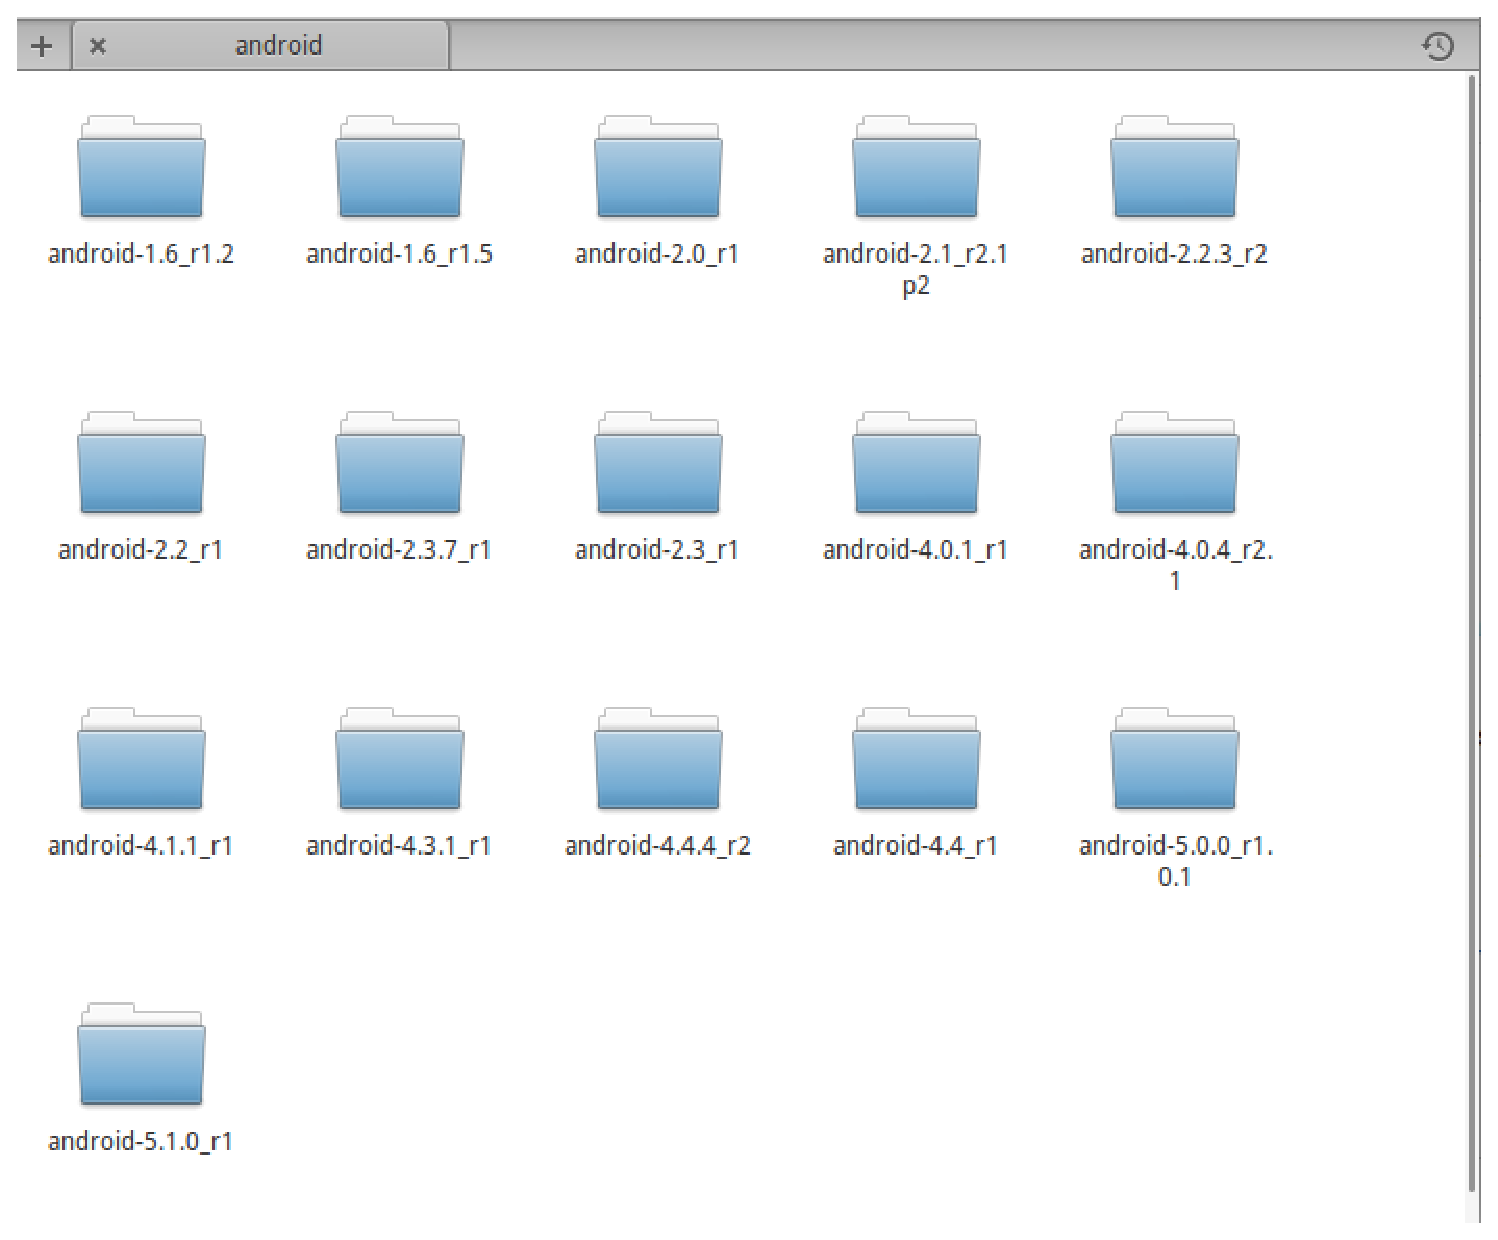
\includegraphics [keepaspectratio=true,scale=0.35]{figuras/folder.eps}
\caption{Diretório onde foram armazenadas cada versão a ser analisada}
\label{folder}
\end{figure}

O restante dos diretórios do AOSP contém desde adaptações de bibliotecas para o Android como o bionic, até código fonte para o \textit{Android Run Time} (ART), que substituiu a dalvik nas ultimas versões do sistema (especificamente desde as versões de \textit{codename Lollipop}), e também códigos de baixo nível específicos para alguns dispositivos. Também existem diretórios para projetos externos ao Android, utilizados pelo mesmo, como o SQLite e outros projetos externos. O kernel utilizado no sistema também tem o seu diretório nessa hierarquia, assim como os aplicativos nativos. A estrutura completa do AOSP não será explorada neste trabalho, mas o conteúdo da pasta raiz pode ser visualizado na Figura~\ref{androidSourceFolders}. A estrutura de diretórios onde foram preparados os códigos para a análise pode ser vista na Figura~\ref{folder}.

Em seguida foi feito o download de cada \textit{tag} em seu diretório, também utilizando a ferramenta \textit{repo}, que realiza um \textit{checkout} de cada subprojeto listado em seu \textit{manifest} através do comando \textit{sync}. O total de espaço em disco ocupado após o download de todas as \textit{TAGS} foi cerca de 10 GB. É importante notar que esse espaço não corresponde apenas a arquivos de código fonte. Após o download e antes de realizar a análise, foi realizada uma filtragem de arquivos na pasta base da análise, removendo todos os arquivos que não correspondessem a código fonte C, C++ ou Java. Da mesma forma, foram removidos todos os diretórios vazios que restaram da deleção dos arquivos, deixando uma árvore de diretórios menor para ser percorrida pela ferramenta de análise, aumentando assim a performance da mesma. O espaço total ocupado pelo código após a filtragem foi de 1,7GB. Não realizar essa remoção não acarretaria em problemas para a análise, entretanto resultaria em um maior tempo necessário para o término na análise.

Além de todas as versões do Android que foram analisadas, o código fonte dos aplicativos do sistema da ultima versão listada para esta análise (\textit{Android Lollipop} 5.1.0 r1) também foi analisado, com o objetivo principal de comparação com o código do sistema. Aplicativos como de email, calculadora e câmera são analisados pela ferramenta Analizo assim como a API de desenvolvimento. São esperados valores relativos semelhantes aos da API do sistema Android.

%TODO rever porcentagens quando tiver todos os dados
No total foram coletados módulos/classes das linguagens C, C++ e Java. Java foi a linguagem mais predominante, com aproximadamente 85\% das amostras, enquanto C++ ocupou pouco mais de 10\% e C pouco mais de 3\%. Embora seja relevante comentar as diferenciações entre as linguagens e seus paradigmas para algumas métricas,  não há necessidade de separação entre os valores para linguagem C, procedural, e linguagens Java/C++, orientadas a objetos, uma vez que, dadas as proporções das mesmas apresentadas nos dados, não há relevância estatística para tal. Entretanto em algumas métricas algumas observações teóricas possam ser ressaltadas, embora, mais uma vez, não haja implicação substancial no resultados gerais apresentados.

\section{Análise de dados}

Após o download de todas as versões escolhidas, foi utilizada a ferramenta Analizo\footnote{\url{http://www.analizo.org/}}  para análise estática de código e coleta de métricas. Um dos motivos da escolha do sistema Debian foi a facilidade de instalação da ferramenta. O Analizo é uma ferramenta livre e extensível para análise de código com suporte a várias linguagens, incluindo Java, que será o foco da análise neste trabalho. Uma grande quantidade de métricas são coletadas pela ferramenta, embora apenas algumas sejam utilizadas para esta análise. Foram coletadas essencialmente métricas de código fonte orientado a objetos. São métricas desse tipo que melhor refletem as decisões arquiteturais ou de design aplicadas durante o desenvolvimento do sistema, como discutido no Capítulo~\ref{cap:metricas}.

Neste trabalho, foi utilizada a funcionalidade de \textit{batch} do Analizo, de forma a coletar métricas de todas as \textit{tags} de uma só vez. A saída da ferramenta é um arquivo CSV para cada projeto ou versão a ser analisada, assim como um arquivo CSV que centraliza os valores de cada métrica a nível de projeto para cada um dos projetos/versões. Isso pode ser interessante quanto utilizado com o mesmo projeto em diferentes versões para verificar o avanço de algumas métricas juntamente com a evolução do sistema.

O resultado da análise de cada projeto contém os valores parciais das métricas para cada arquivo Java que foi analisado pela ferramenta. No total são 16 arquivos CSV contendo cada um as métricas para todas as classes de 1 versão do sistema. O arquivo CSV que contém todas as métricas unificadas para todos os projetos não será utilizado neste trabalho. 

%É importante verificar a variabilidade e os limites de cada uma das métricas e sua evolução desde a primeira versão analisada. Essa verificação dos dados é uma etapa essencial para a escolha de um método estatístico ou de aprendizado de máquina que pode vir a ser utilizado para identificação de padrões e correlações, ou predição de valores. É necessário conhecer o domínio de cada métrica, seus valores médios, mínimos e máximos, para poder realizar a normalização dos dados, caso necessário, e poder analisá-los de forma unificada.

As métricas finais escolhidas foram capturadas pela ferramenta Analizo e estão listadas a seguir:

\begin{itemize}
\item ACCM - \textit{Average Cyclomatic Complexity per Method}
\item AMLOC - \textit{Average Method Lines Of Code}
\item ACC - \textit{Afferent Connections per Class}
\item COF - \textit{Coupling Factor}
\item DIT - \textit{Depth in Inheritance Tree}
\item LCOM4 - \textit{Lack of Cohesion in Methods}
\item NOC - \textit{Number of Children}
\item RFC - \textit{Response For a Class}
\end{itemize}


Essas métricas foram coletadas para cada classe presente em cada versão do Android analisada. Cada uma das versões contém milhares de classes/módulos a serem computados, e essa grande quantidade de classes ajuda a compensar o pequeno número de versões do sistema que foi utilizado, pois como as métricas são calculadas por classe, foi gerada uma quantidade significativa de amostras para cada TAG do sistema.

Para a análise de código fonte em C, que é uma linguagem estruturada, com essas métricas orientadas a objetos, algumas observações devem ser ressaltadas: na ferramenta analizo, em vez de classes, são considerados módulos, e as funções são utilizadas como métodos\cite{meirelles2013}. Embora seja uma abordagem relativamente eficaz para o cálculo das métricas OO, os valores de algumas métricas podem ser bastante distintos das mesmas métricas calculadas para as linguagens que realmente utilizam o paradigma orientado a objetos. No Capítulo~\ref{cap:resultados} serão discutidas, no contexto deste trabalho, as variações de valores para algumas métricas quando analisados nesses diferentes paradigmas. Os valores para C++ e Java já se apresentam similares por utilizarem o mesmo paradigma e portanto terem funcionamento semelhante.
%TODO citar referencia original pag 48

Antes de prosseguir com a utilização dos dados, foi preciso executar uma correção dos dados, pois os arquivos CSV de saída continham classes/módulos com parâmetros de tipos genéricos que utilizam vírgula em sua declaração, comprometendo a formatação correta do arquivo CSV, que utiliza vírgula como separador de valores. Esse problema fazia com que algumas linhas fossem calculadas com mais valores do que deveriam conter, uma vez que as vírgulas adicionais empurravam os valores para a direita e os últimos eram então ignorados. A correção de dados então se resumiu em identificar essas amostras que continham vírgulas e remover as vírgulas adicionais. Esses dados corrigidos então foram armazenados em um diretório a parte para utilização nos estágios seguintes.

Após essa captura de todas as métricas, foram calculados, utilizando linguagem R, os percentis de cada métrica para cada versão do sistema analisada. Cada percentil é a centésima parte dos dados ordenados de forma crescente, ou seja, cada percentil contém 1\% dos dados sendo que o primeiro contém as amostras com menor valor. Esses valores representam nada mais que a frequência cumulativa para cada valor. Isso quer dizer que, para o 90º percentil com um valor de 500, por exemplo, 90\% das amostras apresentam o valor menor ou igual a 500. Como essa frequência cumulativa é calculada em cima dos dados ordenados, a mediana pode ser encontrada no 50º percentil.

Os percentis que foram armazenados foram: 1, 5, 10, 25, 50, 75, 90, 95 e 99, além do menor valor e do máximo valor. Esses dados foram posteriormente reunidos em um arquivo em separado para cada métrica contendo os percentis daquela métrica calculados para cada uma das versões do sistema. A Tabela~\ref{exemplo_percentis} contém um exemplo desse resultado demonstrado para a métrica de complexidade ciclomática coletada do código fonte do sistema Android em várias versões. Os dados coletados para aplicativos foram reunidos da mesma maneira, porém, como só uma versão foi analisada para os aplicativos, em vez de versões, o primeiro valor da tabela é o nome do aplicativo do sistema de onde as métricas foram coletadas.

\begin{table}[!htb]
\scalefont{.7}
%\rowcolors{3}{lightgray}{white}
\begin{tabular}{|l|l|l|l|l|l|l|l|l|l|l|l|l|}
\hline
versão&classes&min&1\%&5\%&10\%&25\%&50\%&75\%&90\%&95\%&99\%&max\\
\hline
android-1.6\_r1.2&5745&0&0&0&0&1&1.11&2&3.45&4.69&9.5&55\\
\hline
android-1.6\_r1.5&5745&0&0&0&0&1&1.11&2&3.45&4.69&9.5&55\\
\hline
android-2.0\_r1&6331&0&0&0&0&1&1.11&2&3.5&4.75&9.74&59\\
\hline
android-2.1\_r2.1p2&6360&0&0&0&0&1&1.12&2&3.5&4.8&9.88&60\\
\hline
android-2.2\_r1&7352&0&0&0&0&1&1.07&2&3.74&5.28&12&99\\
\hline
android-2.2.3\_r2&7358&0&0&0&0&1&1.07&2.02&3.75&5.26&12&99\\
\hline
android-2.3\_r1&8093&0&0&0&0&1&1&2.07&4&5.82&12.83&99\\
\hline
android-2.3.7\_r1&8240&0&0&0&0&1&1&2.08&4&5.8&12.76&99\\
\hline
android-4.0.1\_r1&11709&0&0&0&0&1&1&2.13&4&6&17&94.33\\
\hline
android-4.0.4\_r2.1&11851&0&0&0&0&1&1&2.11&4&6&17&94.33\\
\hline
android-4.1.1\_r1&14115&0&0&0&0&1&1&2&3.86&5.78&16&99.4\\
\hline
android-4.3.1\_r1&15472&0&0&0&0&1&1&2&3.62&5.23&12&120.4\\
\hline
android-5.1.0\_r1&20129&0&0&0&0&1&1&2&3.5&5&11&158.6\\
\hline
\end{tabular}

\scalefont{.7}
\caption{Percentis para os valores de complexidade ciclomática nas versões do Android analisadas}
\label{exemplo_percentis}
\end{table} 

%TODO linkar grafico de demonstração
Com esses arquivos em mãos com os valores de vários percentis para cada métrica nas diversas versões, podem então ser gerados gráficos para melhor visualizar a evolução de cada métrica juntamente com a evolução do sistema. A figura XXXXX apresenta um gráfico de área contendo os valores da métrica XXXXX para cada versão analisada. Fica bem claro o aumento/diminuição(XXXXX) dos valores da métrica para as versões mais recentes do Android. Detalhes da interpretação dos resultados serão discutidos no Capítulo~\ref{cap:resultados}.

Alguns outros gráficos também podem ser gerados a partir dos dados completos, com os valores de cada métrica para cada classe. Gráficos como o histograma, demonstrando os valores mais frequentes, e o boxplot, que ajuda a verificar valores mais discrepantes do restante da amostra, são bastante úteis para a análise dos dados coletados. A figura XXXXX é um boxplot para a métrica XXXXX plotado com todos os dados do sistema. Pode-se perceber claramente que os valores XXX são muito frequentes enquanto os demais são menos frequentes, sendo que alguns são valores atípicos nessas amostras. Outliers, que são esses valores discrepantes, devem ser identificados e removidos para não gerar ruído na interpretação dos dados. Por esse motivo, as amostras mais utilizadas nas análises serão em geral até o 95º percentil. Assim como ~\citeonline{meirelles2013}, os resultados das análises discutidos no Capítulo~\ref{cap:resultados} serão em função dos percentis 75, 90 e 95, correspondendo a valores muito frequentes, frequentes e pouco frequentes, respectivamente. A utilização de 95\%, embora não inclua todas as amostras, ainda resulta em uma boa amostra estatística, uma vez que, como os valores estão ordenados, boa parte desses 5\% restantes são valores discrepantes que podem interferir negativamente na análise correta dos dados.

%TODO incluir interpretação dos dados no quisito regressão linear/polinomial. Comentar o que é necessário ser feito, e como, para fazer a regressão. Mostrar gráficos que demonstram BEM os outliers a serem removidos, explicar pq's e métodos utilizados.

